\documentclass[10pt,aspectratio=169]{beamer}

\usetheme{Madrid}
\usecolortheme{whale}
\usepackage[utf8]{inputenc}
\usepackage[T1]{fontenc}
\usepackage[french]{babel}
\usepackage{lmodern}
\usepackage{booktabs}
\usepackage{amssymb}
\usepackage{graphicx}

\graphicspath{{figs/}}
\setbeamertemplate{navigation symbols}{}
\setbeamerfont{block title}{size=\small}

\title[Absentéisme au travail]{Absentéisme au travail\\\small Séries temporelles \& Classification}
\author[Groupe]{Berthelot Samuel \and Maeva Ange Koumo}
\institute[]{Time Series Analysis}

\begin{document}

\begin{frame}[plain]\titlepage\end{frame}

%======================================================
\begin{frame}{Plan}
\begin{enumerate}\small
  \item Contexte \& problématique
  \item Décomposition (tendance / saisonnalité)
  \item Stationnarité \& différenciation
  \item ACF / PACF
  \item Prévision : modèles \& résultats
  \item Diagnostic des résidus
  \item Effet du jour de la semaine
  \item Classification : cadre
  \item Comparaison des modèles
  \item Séparabilité (PCA) \& erreurs
  \item Variables clés \& conclusion
\end{enumerate}
\vspace{0.5em}
\centering\small Jeu de données UCI \#445 - 740 absences, transporteur brésilien (2007--2010).
\end{frame}

%======================================================
\section{Séries temporelles}

\begin{frame}{1. Contexte \& problématique}
\begin{columns}[c]
\begin{column}{0.5\textwidth}
\begin{block}{Deux questions}\small
\begin{itemize}
  \item \textbf{Prévision} : anticiper le volume mensuel d'heures d'absence ?
  \item \textbf{Explication} : prédire qu'une absence sera \textbf{longue} ?
\end{itemize}
\end{block}
\small
\begin{itemize}
  \item Pas de date $\rightarrow$ index mensuel reconstruit.
  \item \textbf{Série de 37 points} (2007--2010).
\end{itemize}
\end{column}
\begin{column}{0.5\textwidth}
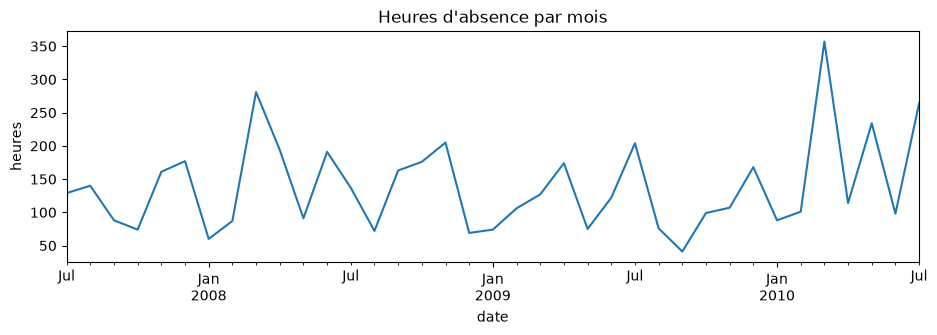
\includegraphics[width=\linewidth]{serie}
\end{column}
\end{columns}
\end{frame}

\begin{frame}{2. Décomposition saisonnière - Additif ($X = T + S + R$)}
\begin{columns}[c]
\begin{column}{0.4\textwidth}\small
\begin{itemize}
  \item Décomposition par \textbf{moyenne mobile}.
  \item $T$ tendance, $S$ saison, $R$ résidu (bruit).
  \item Saison d'amplitude $\approx \pm 50$--$75$~h\dots
  \item \dots du \textbf{même ordre} que les résidus ($\pm 50$--$70$~h).
  \item[$\Rightarrow$] la saison \alert{ne domine pas le bruit}.
\end{itemize}
\end{column}
\begin{column}{0.6\textwidth}
\centering 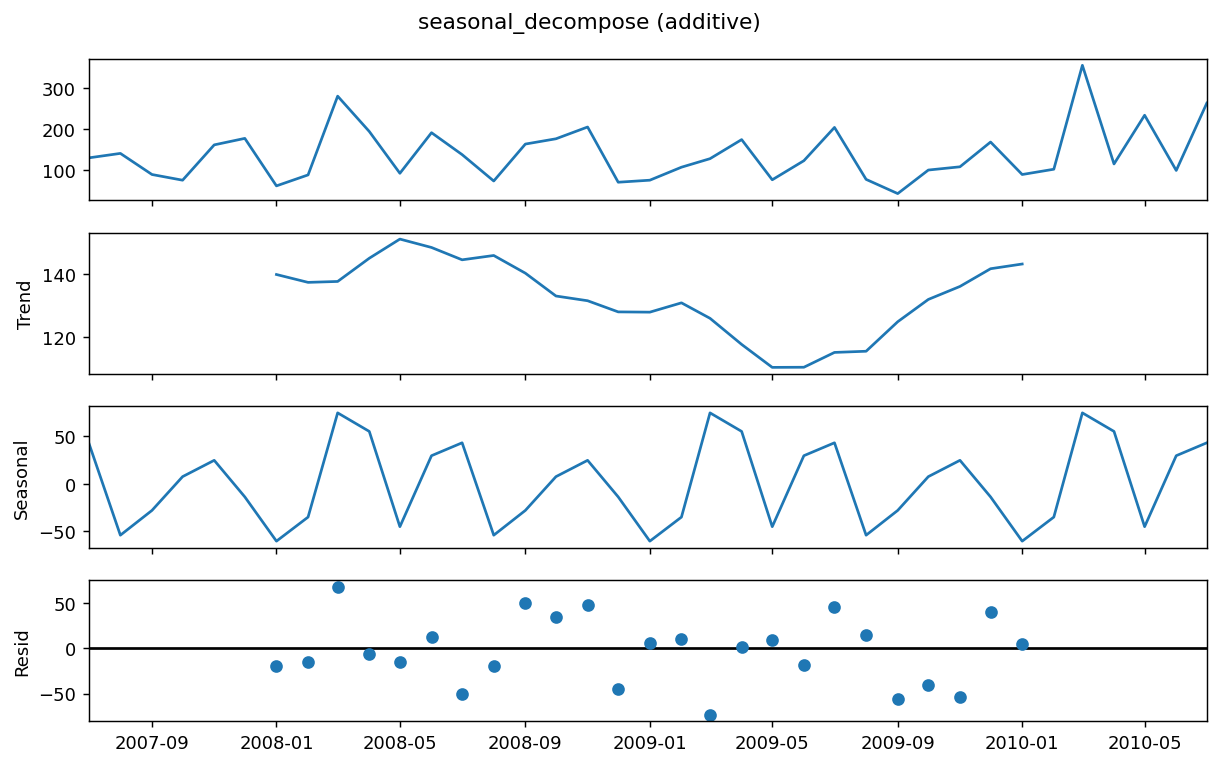
\includegraphics[width=\linewidth]{decomp}
\end{column}
\end{columns}
\end{frame}

\begin{frame}{2. Décomposition saisonnière - Multiplicatif ($X = T \cdot S \cdot R$)}
\begin{columns}[c]
\begin{column}{0.4\textwidth}\small
\begin{itemize}
  \item Même effet de \textbf{tendance} que l'additif.
  \item Facteur saisonnier $\in [0{,}6\,;\,1{,}55]$.
  \item Même forme \textbf{répétée}.
  \item[$\Rightarrow$] effet visible mais \alert{pas écrasant}.
\end{itemize}
\end{column}
\begin{column}{0.6\textwidth}
\centering 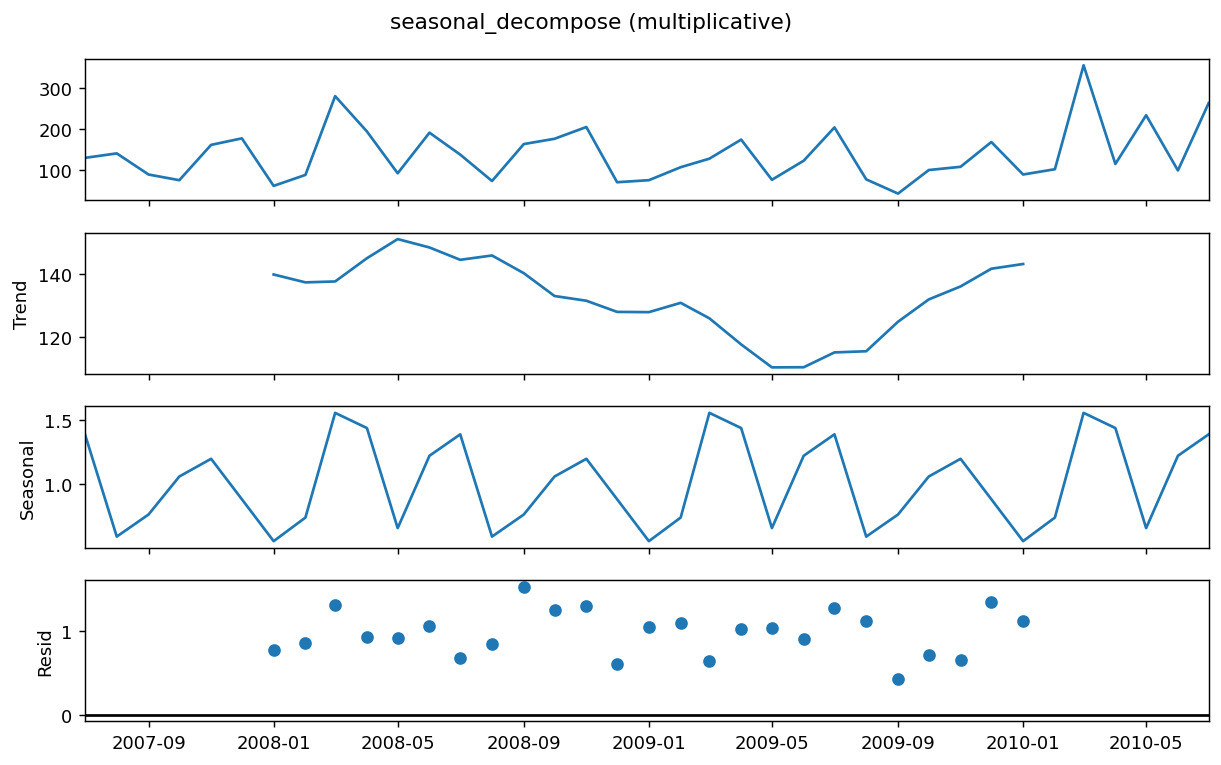
\includegraphics[width=\linewidth]{decomp1}
\end{column}
\end{columns}
\end{frame}

\begin{frame}{2. Décomposition saisonnière - STL (Loess)}
\begin{columns}[c]
\begin{column}{0.4\textwidth}\small
\begin{itemize}
  \item Tendance STL = \textbf{droite}, vs creuse (additif/multi) : \alert{désaccord sur la tendance}.
  \item Profil saisonnier \alert{instable} $\rightarrow$ saison faible et incertaine.
  \item 3 cycles de 12 mois seulement $\rightarrow$ trop peu fiable.
  \item[$\Rightarrow$] saison pas assez robuste, \textbf{SARIMA non justifié}.
\end{itemize}
\end{column}
\begin{column}{0.6\textwidth}
\centering 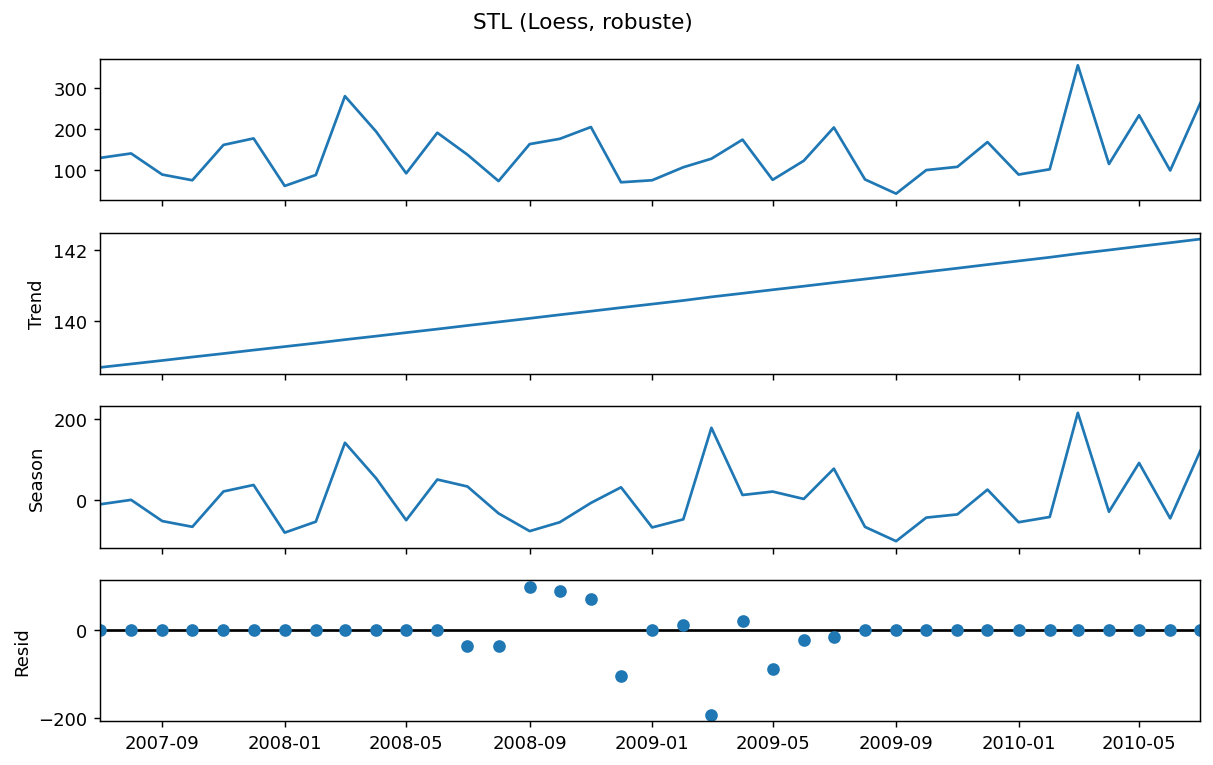
\includegraphics[width=\linewidth]{decomp2}
\end{column}
\end{columns}
\end{frame}

\begin{frame}{3. Stationnarité \& différenciation}
\begin{columns}[c]
\begin{column}{0.5\textwidth}
\begin{block}{ADF \& KPSS (hypothèses opposées)}\small
\textbf{ADF} $p=0{,}000$ (rejette racine unitaire) \textbf{et} \textbf{KPSS} $p=0{,}100$ (ne rejette pas)
$\Rightarrow$ \alert{stationnaire} $\Rightarrow d=0$.
\end{block}
\small
\begin{itemize}
  \item Différenciation $\nabla=(1-B)$ testée par vérification :
  \item écart-type $69\rightarrow102$, autocorr. lag~1 $\rightarrow-0{,}47$
  \item[$\Rightarrow$] \alert{sur-différenciation} $\rightarrow$ on garde $d=0$.
\end{itemize}
\end{column}
\begin{column}{0.5\textwidth}
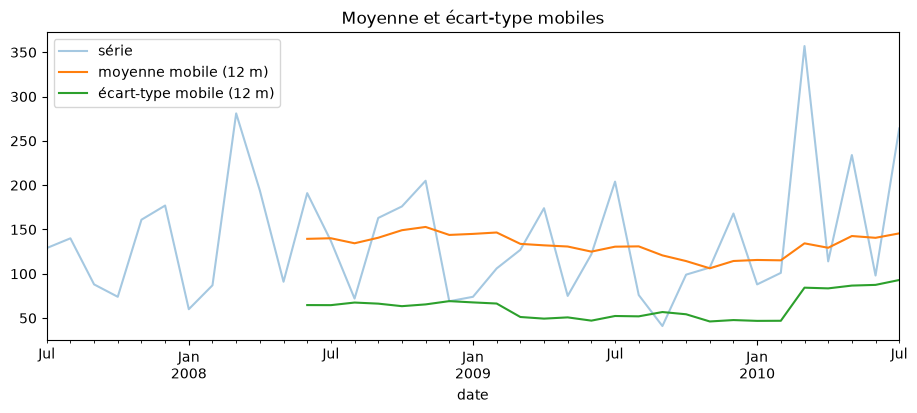
\includegraphics[width=\linewidth]{stationnarite}
\end{column}
\end{columns}
\end{frame}

\begin{frame}{4. ACF / PACF}
\begin{columns}[c]
\begin{column}{0.36\textwidth}\small
\textbf{Série brute}
\begin{itemize}
  \item décroissance immédiate $\rightarrow$ stationnaire ;
  \item \textbf{aucun pic au lag 12} $\rightarrow$ pas de saison ;
  \item[$\Rightarrow$] \alert{proche d'un bruit blanc}.
\end{itemize}
\textbf{Différenciée}
\begin{itemize}
  \item pic négatif lag~1 ($-0{,}47$) $\rightarrow$ \alert{sur-différenciation}.
\end{itemize}
\end{column}
\begin{column}{0.64\textwidth}
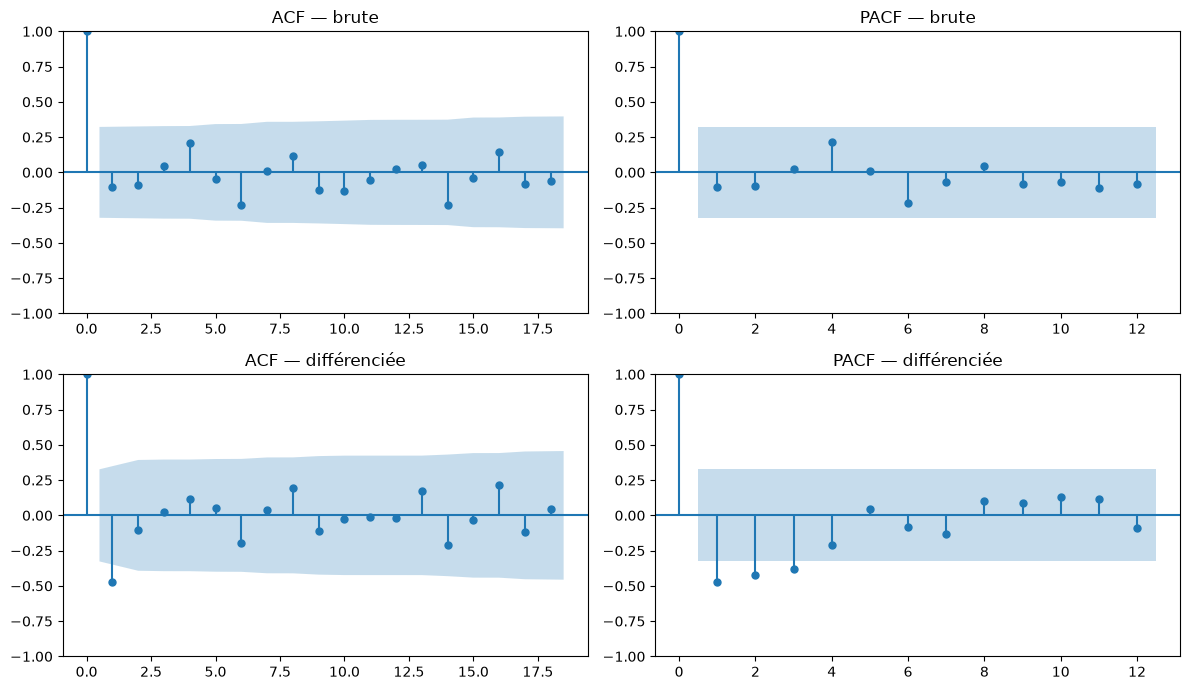
\includegraphics[width=\linewidth]{acfpacf}
\end{column}
\end{columns}
\end{frame}

\begin{frame}{4bis. Mois de pic : quels motifs ?}
\begin{columns}[c]
\begin{column}{0.38\textwidth}\small
\begin{itemize}
  \item Mois le plus chargé : \textbf{mars 2010}.
  \item Top en heures \textbf{ex æquo} :
  \begin{itemize}\small
    \item \alert{Maladies de la peau} - 112~h ;
    \item \alert{Traumatismes / causes externes} - 112~h.
  \end{itemize}
  \item[$\Rightarrow$] pic = \textbf{mélange accidents + maladies}, pas une cause unique.
\end{itemize}
\vspace{0.4em}
{\footnotesize\textit{Hypothèse contextuelle} : compatible avec la \textbf{saison des pluies} brésilienne de 2010 (accidents + infections cutanées ; épidémie de dengue). Non prouvé - année reconstruite.}
\end{column}
\begin{column}{0.62\textwidth}
\centering 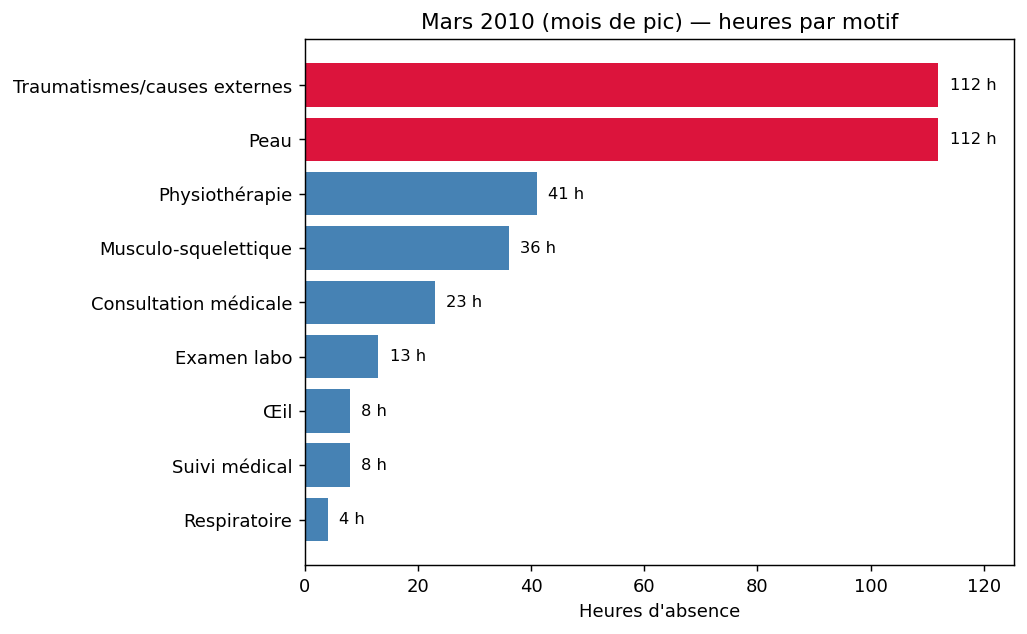
\includegraphics[width=\linewidth]{pic_mars}
\end{column}
\end{columns}
\end{frame}

\begin{frame}{5. Prévision - baselines}
\begin{columns}[c]
\begin{column}{0.52\textwidth}\small
\textbf{Problématique} : anticiper le volume mensuel d'heures d'absence (planification RH).
\begin{itemize}
  \item Split chronologique : \textbf{train 28} / \textbf{test 9} mois.
  \item \textbf{SARIMA} écarté (saison instable) ; \textbf{ARIMA} $=$ ARMA car $d=0$.
  \item Métriques : \textbf{RMSE} (sanctionne les gros écarts) pour classer, \textbf{MAE} (erreur typique en h) pour interpréter.
  \item[$\Rightarrow$] un modèle n'a de valeur que s'il \alert{bat la meilleure baseline}.
\end{itemize}
\end{column}
\begin{column}{0.48\textwidth}
\begin{block}{Baselines}\small
\begin{itemize}
  \item \textbf{moyenne} : moyenne du train ;
  \item \textbf{naïf} : dernière valeur observée ;
  \item \textbf{naïf saisonnier} : valeur à $t-12$.
\end{itemize}
\end{block}
\begin{center}\scriptsize
\begin{tabular}{lcc}
\toprule & MAE & RMSE \\ \midrule
\alert{moyenne} & 71,5 & \alert{98,5} \\
naïf (dernière) & 73,8 & 114,1 \\
naïf saisonnier & 83,2 & 108,3 \\ \bottomrule
\end{tabular}
\end{center}
\centering\small À battre : \alert{moyenne (RMSE 98,5)}.
\end{column}
\end{columns}
\end{frame}

\begin{frame}{5. Prévision - AR($p$) \& MA($q$)}
\begin{columns}[c]
\begin{column}{0.56\textwidth}\small
\begin{block}{AR($p$) - autorégression}\small
Série stationnaire $\rightarrow$ applicable. Ordre $p$ = dernier lag \textbf{PACF} significatif ($-0{,}48$) $\rightarrow$ \textbf{AR(2)}.
\end{block}
\begin{block}{MA($q$) - moyenne mobile}\small
Même principe, ordre $q$ = dernier lag \textbf{ACF} significatif $\rightarrow$ \textbf{MA(2)}. Estimé par MLE (\texttt{ARIMA(0,0,q)}).
\end{block}
\end{column}
\begin{column}{0.44\textwidth}
\begin{center}\small
\begin{tabular}{lcc}
\toprule & MAE & RMSE \\ \midrule
\alert{AR(2)} & 70,6 & \alert{96,3} \\
MA(2) & 70,6 & 97,7 \\ \midrule
moyenne & 71,5 & 98,5 \\ \bottomrule
\end{tabular}
\end{center}
\vspace{0.4em}
\small Les deux battent la moyenne ; \alert{AR(2)} en tête (RMSE 96,3).
\end{column}
\end{columns}
\end{frame}

\begin{frame}{5. Prévision - ARMA($p,0,q$) \& résultats}
\begin{columns}[c]
\begin{column}{0.42\textwidth}\small
\begin{itemize}
  \item \textbf{ARMA($p,0,q$)} : balayage de la grille $(p,q)$, sélection par \textbf{BIC}.
  \item BIC pénalise plus que l'AIC ($\ln T$ vs $2$) $\rightarrow$ plus \textbf{parcimonieux}.
  \item BIC minimal $\rightarrow$ \textbf{ARMA(0,2)} $=$ MA(2).
  \item[$\Rightarrow$] meilleur RMSE global : \alert{AR(2) $=$ 96,3}.
\end{itemize}
\vspace{0.2em}
{\footnotesize Gain de $\sim\!2\%$ sur la moyenne (96,3 vs 98,5) : série \alert{proche d'un bruit blanc}, peu de dynamique exploitable.}
\vspace{0.2em}
\end{column}
\begin{column}{0.58\textwidth}
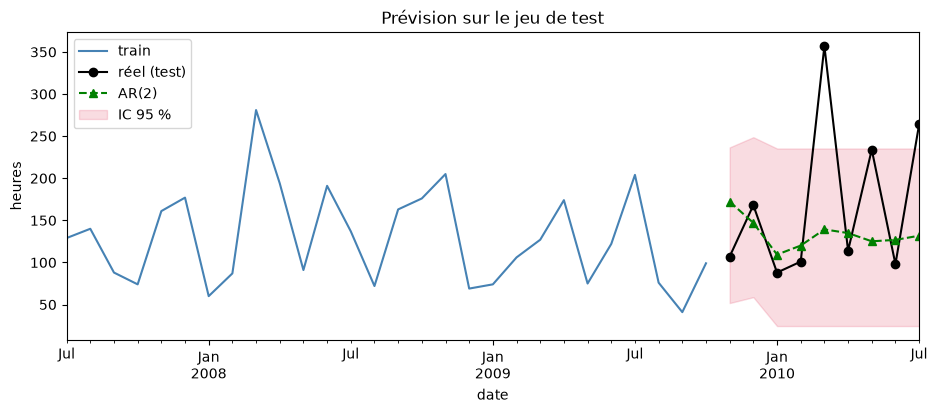
\includegraphics[width=\linewidth]{prev_test}
\end{column}
\end{columns}
\end{frame}

\begin{frame}{6. Diagnostic des résidus (Box--Jenkins)}
\begin{columns}[c]
\begin{column}{0.42\textwidth}\small
\begin{itemize}
  \item Modèle validé si résidus $=$ bruit blanc.
  \item ACF des résidus \textbf{plate}, centrés sur 0.
  \item \textbf{Ljung-Box} (H0 : pas d'autocorr.) : $p>0{,}05$ $\rightarrow$ \alert{bruit blanc}.
\end{itemize}
\begin{center}\scriptsize
\begin{tabular}{ccc}
\toprule
lag & \texttt{lb\_stat} & \texttt{lb\_pvalue} \\ \midrule
6  & 1,802 & \alert{0,937} \\
12 & 6,744 & \alert{0,874} \\ \bottomrule
\end{tabular}
\end{center}
\begin{block}{Conclusion}\small
Série $\approx$ bruit blanc $\rightarrow$ \textbf{pivot} vers l'analyse explicative.
\end{block}
\end{column}
\begin{column}{0.58\textwidth}
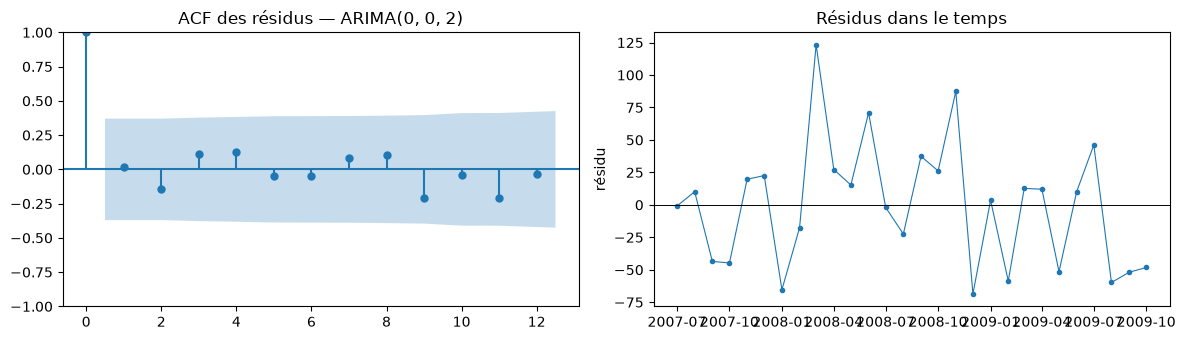
\includegraphics[width=\linewidth]{residus}
\end{column}
\end{columns}
\end{frame}

%======================================================
\section{Analyse explicative}

\begin{frame}{7. Effet du jour de la semaine}
\begin{columns}[c]
\begin{column}{0.44\textwidth}\small
\begin{itemize}
  \item Analyse de l'effet du jour.
  \item \textbf{Nombre} d'absences homogène ; c'est la \textbf{durée} qui varie : lundi \alert{9,2~h} $\rightarrow$ jeudi 4,4~h.
  \item \textbf{Kruskal-Wallis} : $H=10{,}7$, $p=0{,}030$.
  \item[$\Rightarrow$] jour = \alert{prédicteur pertinent}.
\end{itemize}
\end{column}
\begin{column}{0.56\textwidth}
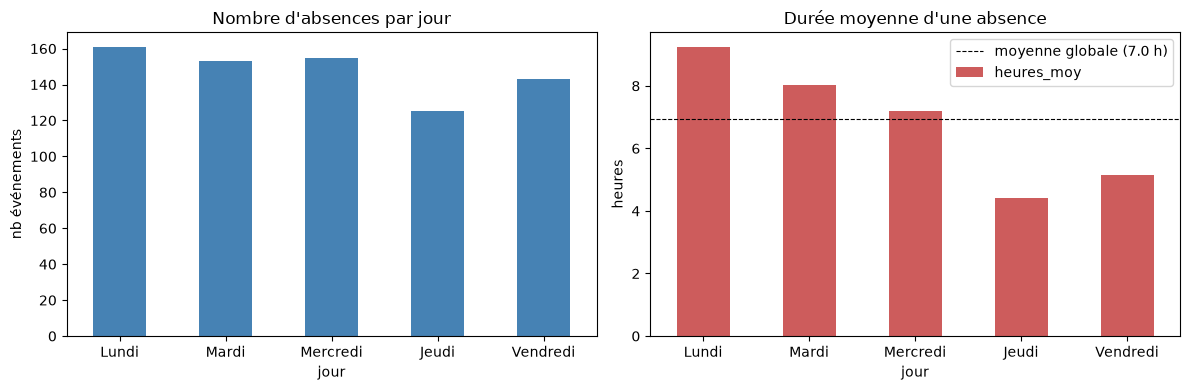
\includegraphics[width=\linewidth]{jour}\\[2pt]
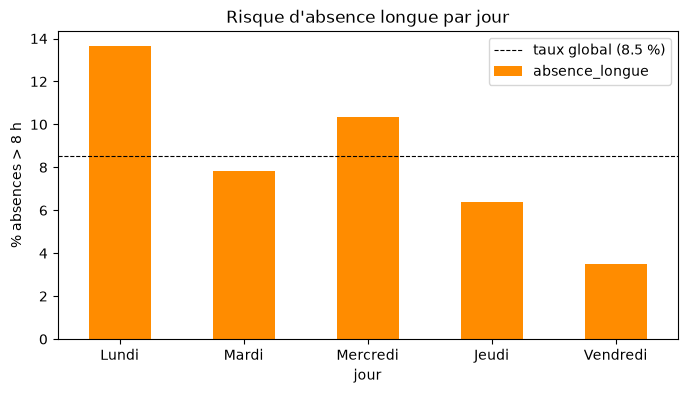
\includegraphics[width=0.62\linewidth]{jour_long}
\end{column}
\end{columns}
\end{frame}

\begin{frame}{8. Classification : cadre}
\begin{block}{Cible : 3 classes de durée}
\textbf{low} ($\leq 4$h, 458) \quad \textbf{mod} (5--8h, 216) \quad \textbf{high} ($>8$h, 63)
\end{block}
\begin{itemize}
  \item Classes \alert{déséquilibrées} $\rightarrow$ \textbf{pas l'accuracy}.
  \item Métriques : \textbf{macro-F1} (classes à poids égal), \textbf{ROC-AUC (ovr)}, balanced accuracy.
  \item Pipeline \texttt{préproc. $\rightarrow$ modèle} (one-hot + standardisation), split stratifié 75/25 + CV 5-fold.
  \item 5 modèles : baseline, régression logistique, arbre de décision, SVM, Random Forest.
\end{itemize}
\end{frame}

\begin{frame}{9. Comparaison des modèles}
\begin{center}
\begin{tabular}{lcccc}
\toprule
Modèle & CV F1-macro & test F1-macro & ROC-AUC (ovr) & bal-acc \\ \midrule
Baseline (majoritaire)        & 0,256 & 0,256 & 0,500 & 0,333 \\
\alert{Régression logistique} & \alert{0,611} & 0,592 & 0,823 & 0,636 \\
Arbre de décision             & 0,518 & 0,467 & 0,639 & 0,470 \\
SVM                           & 0,576 & 0,560 & \alert{0,842} & 0,586 \\
Random Forest                 & 0,595 & 0,581 & 0,838 & 0,584 \\
\bottomrule
\end{tabular}
\end{center}
\begin{itemize}
  \item Tous \alert{loin devant la baseline} (0,26).
  \item Meilleur en \textbf{F1} : régression logistique ; en \textbf{AUC} : SVM. Un modèle \textbf{simple} rivalise.
\end{itemize}
\end{frame}

\begin{frame}{10. Séparabilité (PCA) \& erreurs}
\begin{columns}[c]
\begin{column}{0.5\textwidth}
\centering
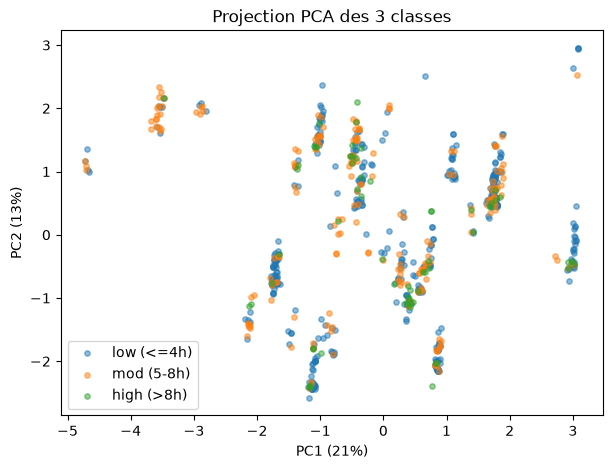
\includegraphics[width=0.92\linewidth]{pca}\\ \tiny classes qui se chevauchent (34\% de variance en 2D)
\end{column}
\begin{column}{0.5\textwidth}
\centering
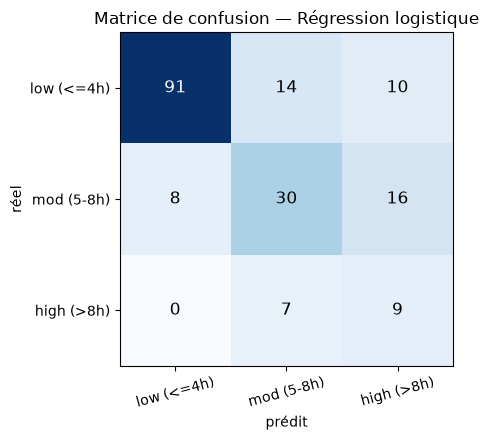
\includegraphics[width=0.82\linewidth]{confusion}
\end{column}
\end{columns}
\vspace{0.3em}
\small\centering
\textbf{low} F1 0,85 \; | \; \textbf{mod} 0,57 (ambiguë) \; | \; \textbf{high} rappel 0,56 / précision 0,26 (rare)
$\;\Rightarrow$ difficulté \alert{intrinsèque aux données}.
\end{frame}

\begin{frame}{11. Variables clés \& conclusion}
\begin{columns}[c]
\begin{column}{0.5\textwidth}
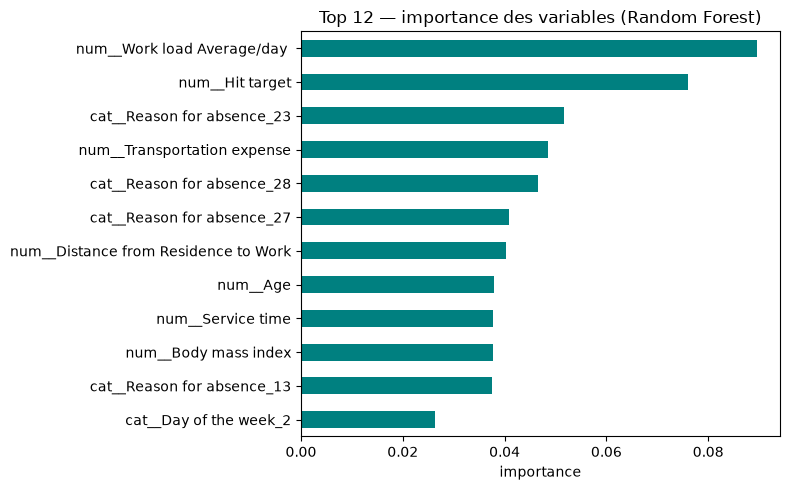
\includegraphics[width=\linewidth]{importances}
\end{column}
\begin{column}{0.5\textwidth}\small
\textbf{Charge de travail} ($\sim9\%$), \textbf{Hit target} ($\sim7{,}6\%$), puis \textbf{motif} ; \textbf{jour} $\sim10\%$ cumulé (confirme §4).
\begin{itemize}
  \item \textbf{Prévision} : série $\approx$ bruit $\rightarrow$ peu fiable.
  \item \textbf{Explication} : absences courtes bien classées ; longues plus dures (rares).
  \item \textbf{Limites} : 37 points, classe \emph{high} rare $\rightarrow$ CV = mesure fiable.
\end{itemize}
\end{column}
\end{columns}
\end{frame}

\begin{frame}[plain]
\centering\Large Merci - Des questions ?
\end{frame}

\end{document}
